\documentclass{beamer}

\usepackage{lmodern}

\usepackage{listings}


\usepackage{algorithm}
\usepackage{algpseudocode}
\usepackage{amsmath}

\usepackage[T2A]{fontenc}
\usepackage[utf8]{inputenc}

\usetheme{Madrid}
\usecolortheme{beaver}

\title[]{Размещение реплик в распределенной\\системе на базе Erlang-процессов}
\author[Быцюк В.В.]{Быцюк Владислав Вячеславович}
\date[]{}

\begin{document}
	\setbeamertemplate{caption}{\raggedright\insertcaption\par}

% Титульный лист
\begin{frame}
	\titlepage
	\begin{center}
		Научный руководитель:\\д.ф.-м.н., профессор В.С. Пилиди\\~\\

		Рецензент:\\к.ф.-м.н., доцент С.А. Гуда\\~\\

		Прикладная математика и информатика

		Кафедра информатики и вычислительного эксперимента
	\end{center}
\end{frame}

% Постановка задачи
\begin{frame}{\LARGE \textbf{Постановка задачи}}
	\begin{itemize}
		\item Реализовать распределенное клиент-серверное приложение для хранения данных на языке программирования Erlang. 
    	\item Реализовать алгоритм размещения реплик объектов в распределенной сети. 
    	\item Провести замеры количества итераций алгоритма и проанализировать полученные результаты.
	\end{itemize}
\end{frame}
	
	
% Основное содержание

\begin{frame}[fragile]{Erlang-процессы}
	\begin{block}{Запуск процесса}
		\begin{lstlisting}[language = erlang] 	
Pid = spawn(Fun).
		\end{lstlisting}
	\end{block}	

	\begin{block}{Отправка сообщения}
		\begin{lstlisting}[language = erlang] 	
Pid ! Message.
		\end{lstlisting}
	\end{block}	

	\begin{block}{Ожидание сообщений}
		\begin{lstlisting}[language = erlang] 	
receive
  Pattern1 -> Expressions1;
  Pattern2 -> Expressions2;
  true     -> Expression3
end
		\end{lstlisting}
	\end{block}	
\end{frame}

\begin{frame}[fragile]{Клиент-серверное приложение}
	\begin{figure}
		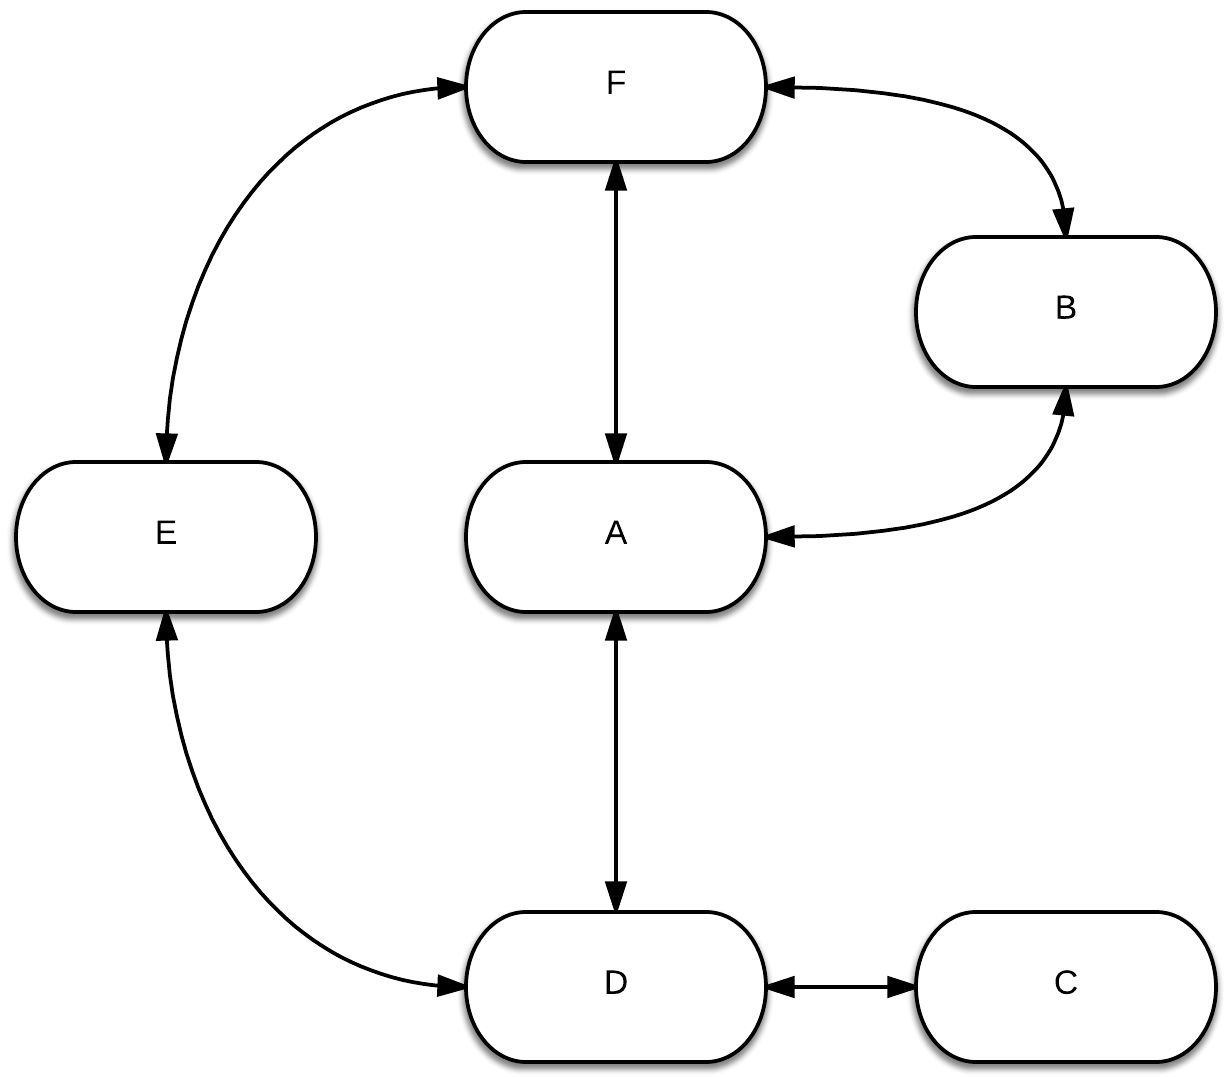
\includegraphics[scale=0.18]{img/example.png}
		\caption{Пример произвольной топологии системы}
	\end{figure}
\end{frame}
	
\begin{frame}[fragile]{Клиент-серверное приложение}
	\begin{figure}
		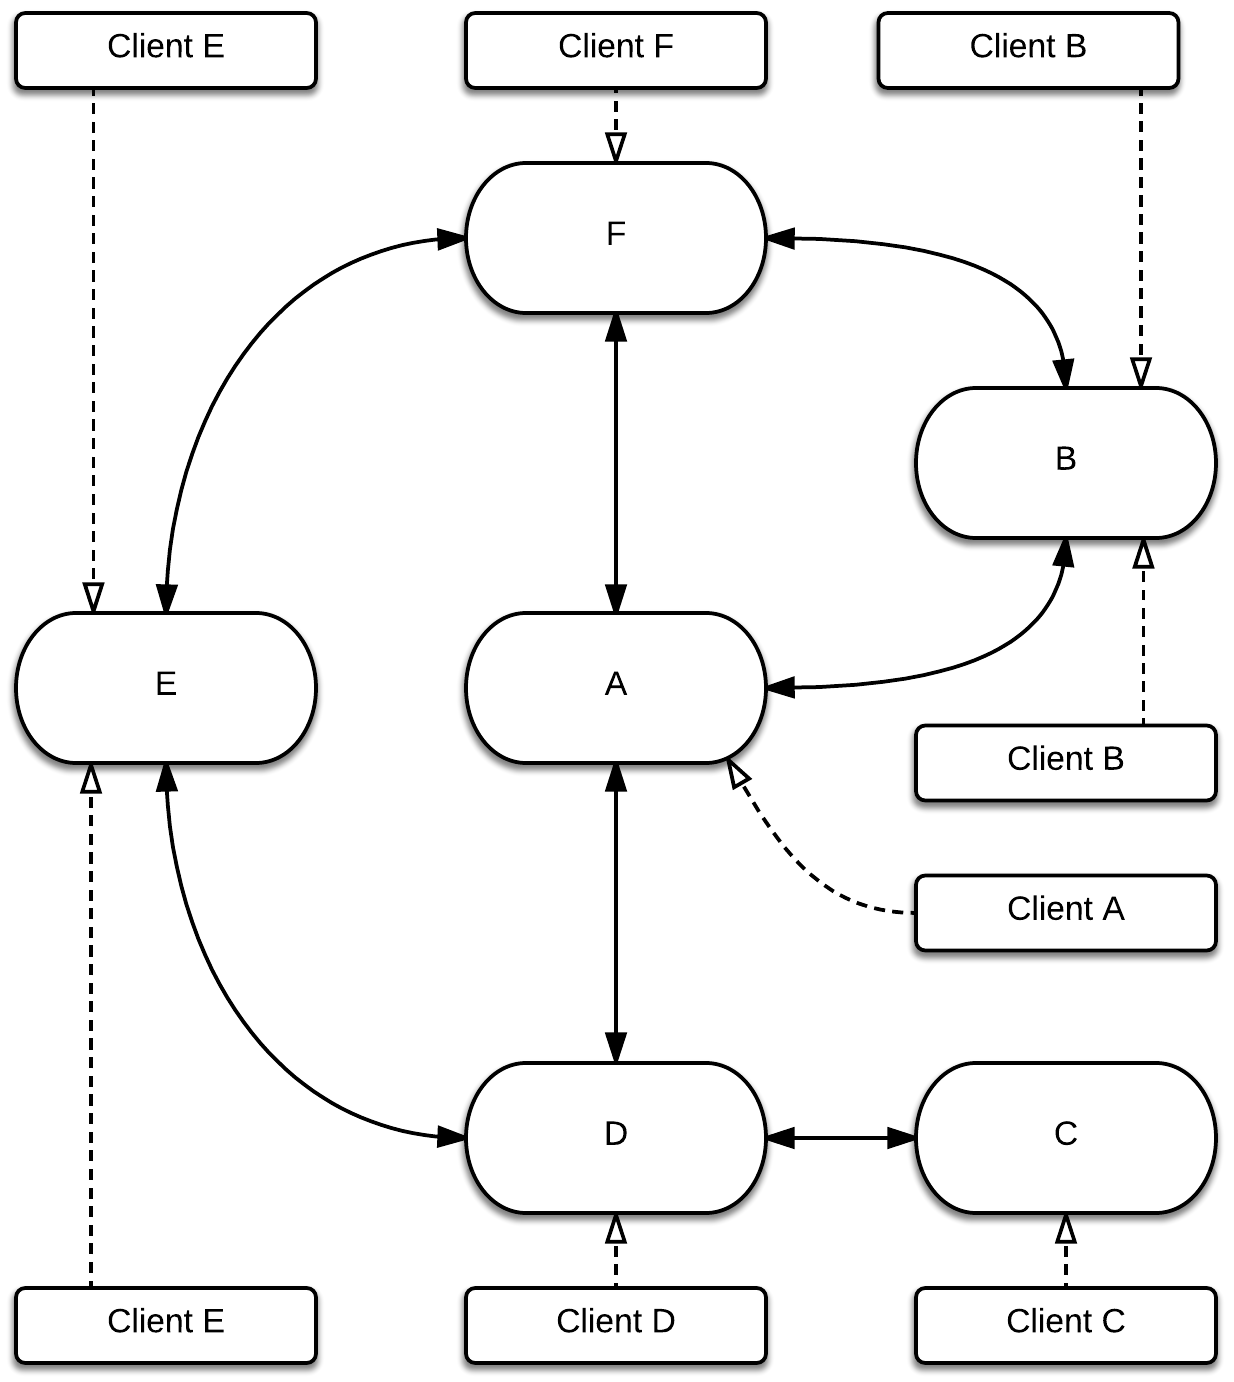
\includegraphics[scale=0.14]{img/client_ex.png}
		\caption{Пример системы с клиентами}
	\end{figure}
\end{frame}

\begin{frame}[fragile]{Клиент-серверное приложение}
	\begin{figure}
		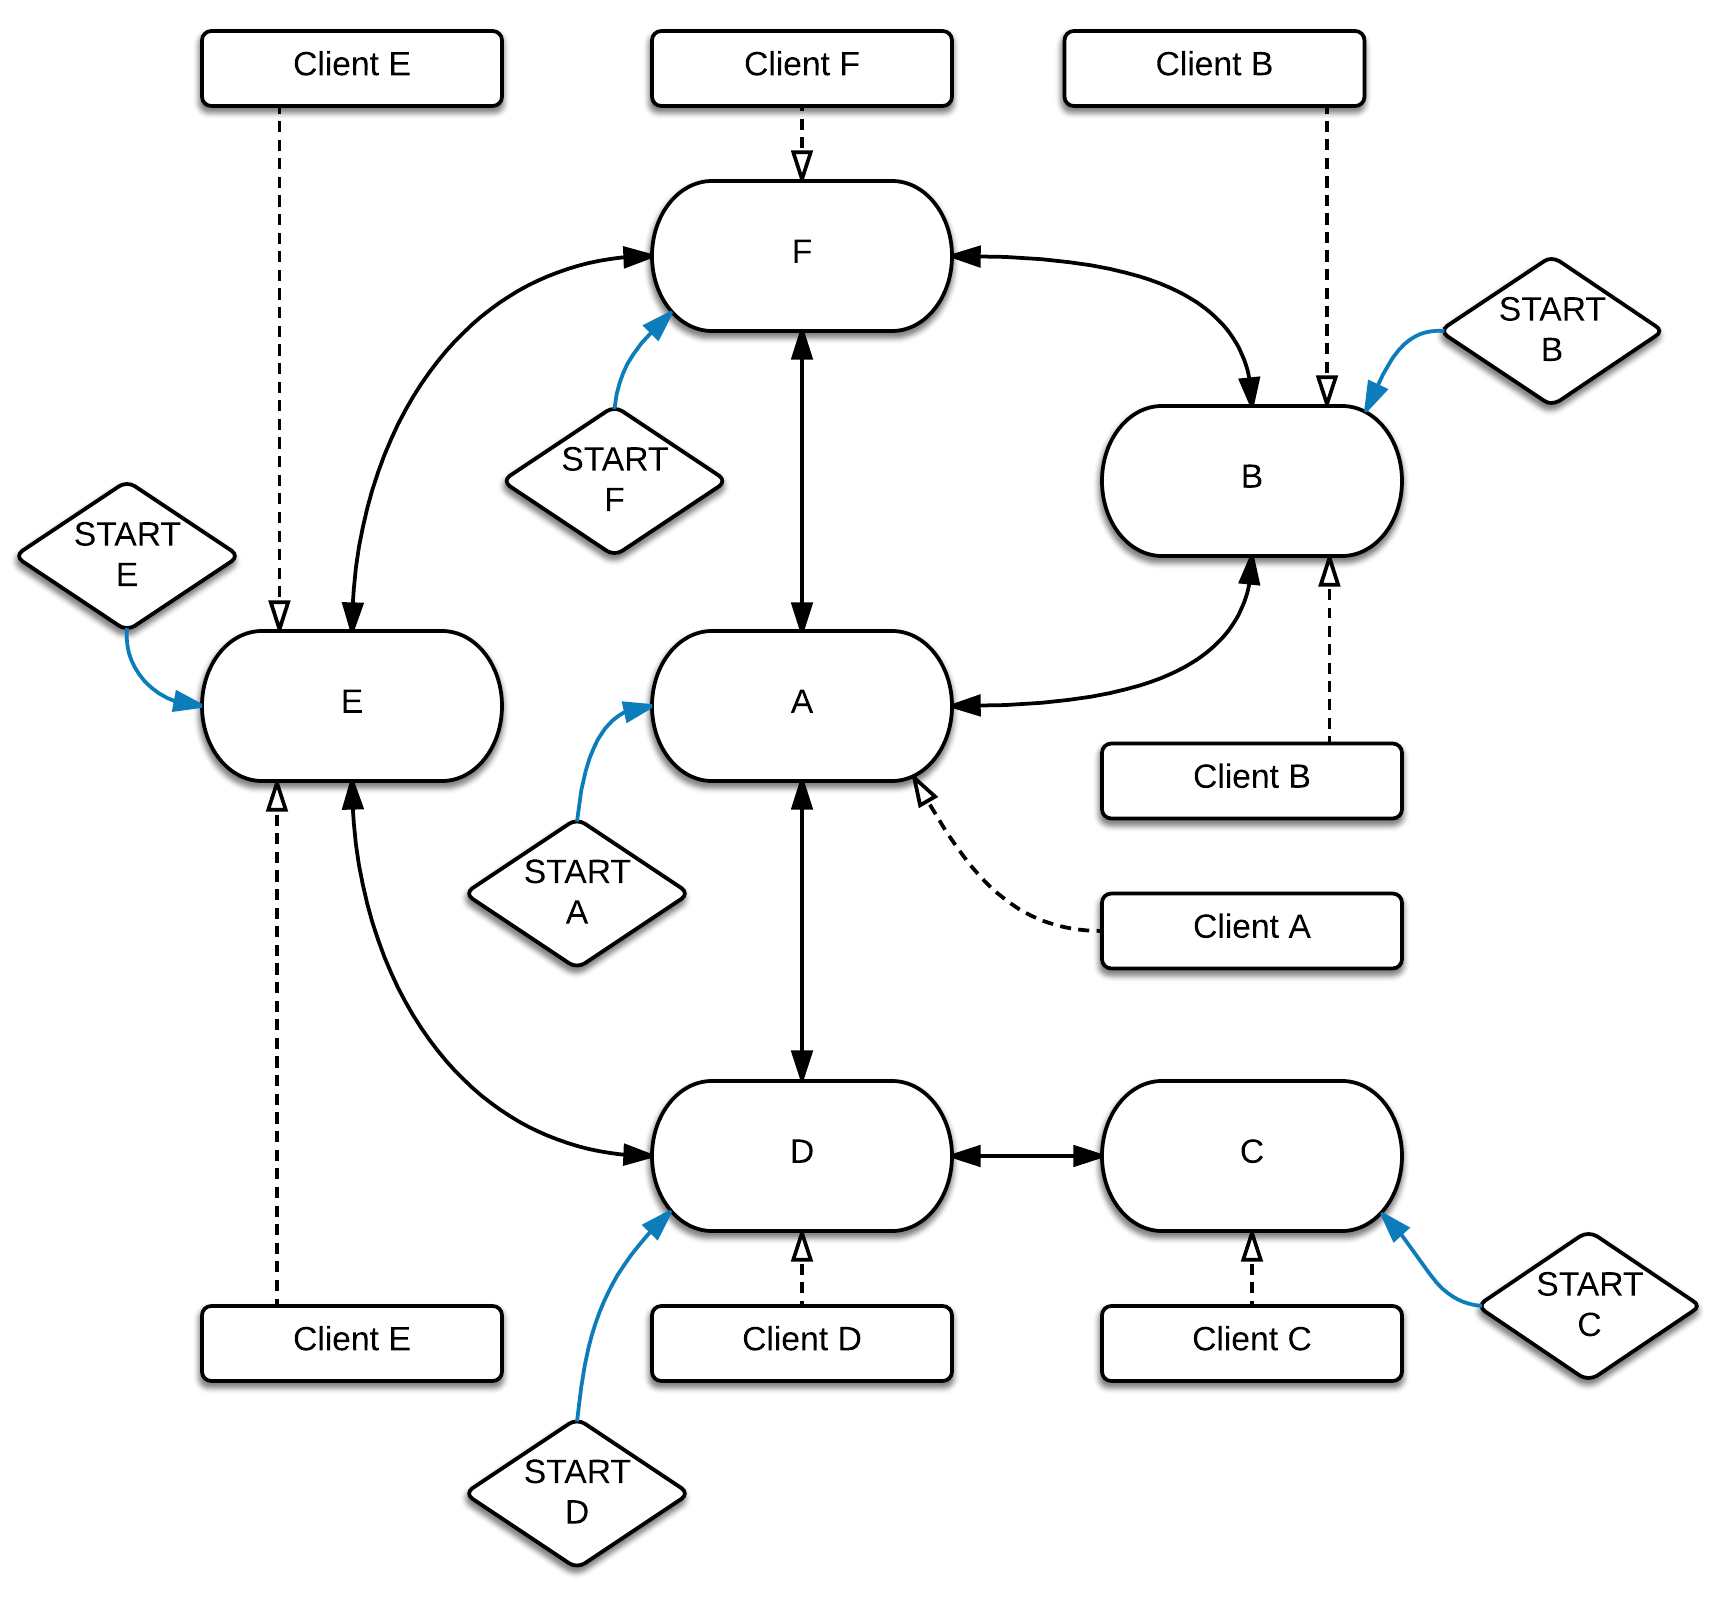
\includegraphics[scale=0.11]{img/start.png}
		\caption{Пример системы с клиентами и процессами запуска}
	\end{figure}
\end{frame}

\begin{frame}[fragile]{Клиент-серверное приложение}
	\begin{figure}
		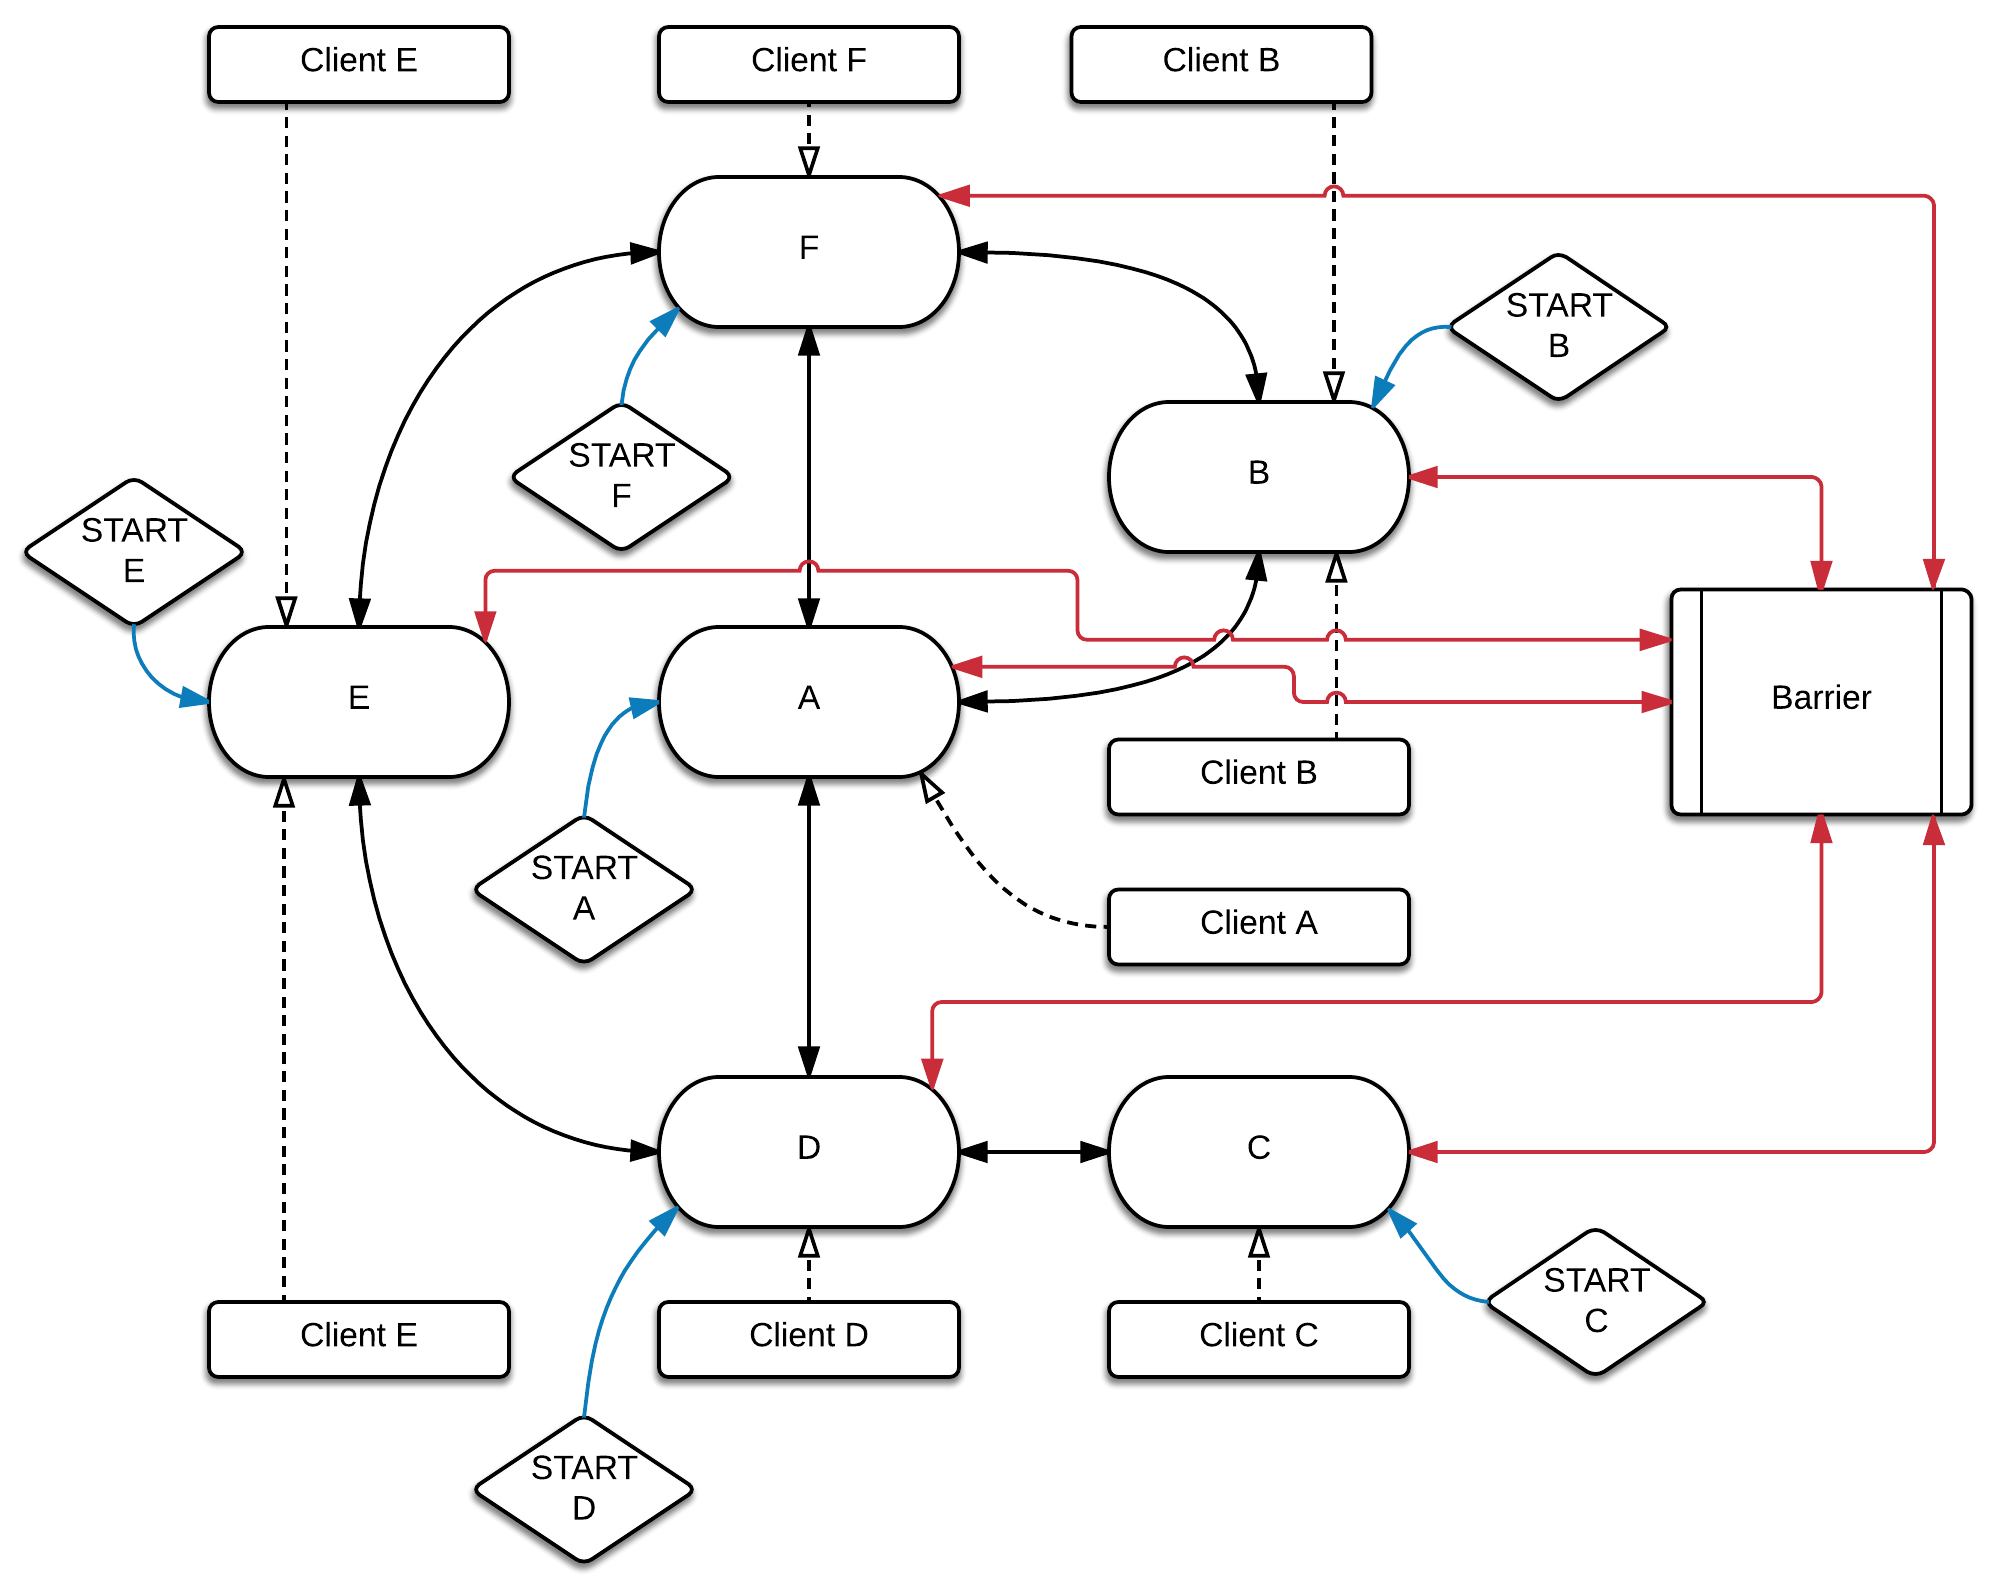
\includegraphics[scale=0.11]{img/bar.png}
		\caption{Пример системы с клиентами, процессами запуска и процессом барьера}
	\end{figure}
\end{frame}

\begin{frame}[fragile]{Основные обозначения}
	$s_1, \ldots, s_m$~---~сервера,\quad$o_1, \ldots, o_n$~---~объекты,\quad$c_1, \ldots, c_m$~---~емкости~серверов\\~\\
	
	$t_l$ --- время доступа к объекту хранящемуся на текущем сервере\\
	$t_r$ --- время доступа к объекту хранящемуся на соседнем сервере\\
	$t_s$ --- время доступа к объекту хранящемуся на удаленном сервере\\~\\

	$rc_j$ --- количество копий объекта $o_j$ на всех серверах\\
	$r_{ij}$ --- количество запросов к объекту $o_j$ с сервера $s_i$\\
	$p_j = \sum_{i=1}^{m} r_{ij}$ --- количество запросов к объекту $o_j$ со всех серверов\\~\\
\end{frame}

\begin{frame}[fragile]{Основные обозначения}
	$X_{ij}$ --- флаг, говорящий о том, размещен ли объект $o_j$ на сервере $s_i$
	\[ 	
		X_{ij} =
		\begin{cases} 
			1 & o_j \in s_i \\ 
			0 & o_j \notin s_i 
		\end{cases}
	\] 
	$ig_{ij}$ --- выгода от вставки объекта $o_j$ на сервер $s_i$
	\[ 	
		ig_{ij} =
		\begin{cases} 
			p_j (t_s - t_r) + r_{ij} (t_r - t_l) 	& rc_j = 0 \\
			r_{ij} (t_r - t_l) 						& X_{ij} = 0, rc_j > 0 \\
			0 										& X_{ij} = 1 
		\end{cases}
	\] 
	$ec_{ij}$ --- стоимость удаления объекта $o_j$ с сервера $s_i$
	\[ 	
		ec_{ij} =
		\begin{cases} 
			0										& X_{ij} = 0 \\
			r_{ij} (t_r - t_l) 						& X_{ij} = 1, rc_j > 0 \\
			p_j (t_s - t_r) + r_{ij} (t_r - t_l)	& X_{ij} = 1, rc_j = 1 
		\end{cases}
	\]
\end{frame}

\begin{frame}[fragile]{Краткое описание алгоритма размещения реплик}
	Алгоритм размещения реплик действует по следующей схеме:
	\begin{enumerate}
		\item Инициализация всех данных необходимых для работы алгоритма на каждом сервере
		\item Нахождение объекта, вставка которого принесет максимальную выгоду на каждом сервере
		\item Коллективное решение, о том какой объект и на каком сервере будет размещен
		\item Размещение выбранного объекта на выбранном сервере, и внесение информации об этом 
			  действии на каждый сервер системы
		\item Переход на шаг 2 до тех пор пока хотя бы на один из серверов возможна вставка объекта
	\end{enumerate}
\end{frame}

\begin{frame}[fragile]{Тестовые испытания}
	\begin{figure}
		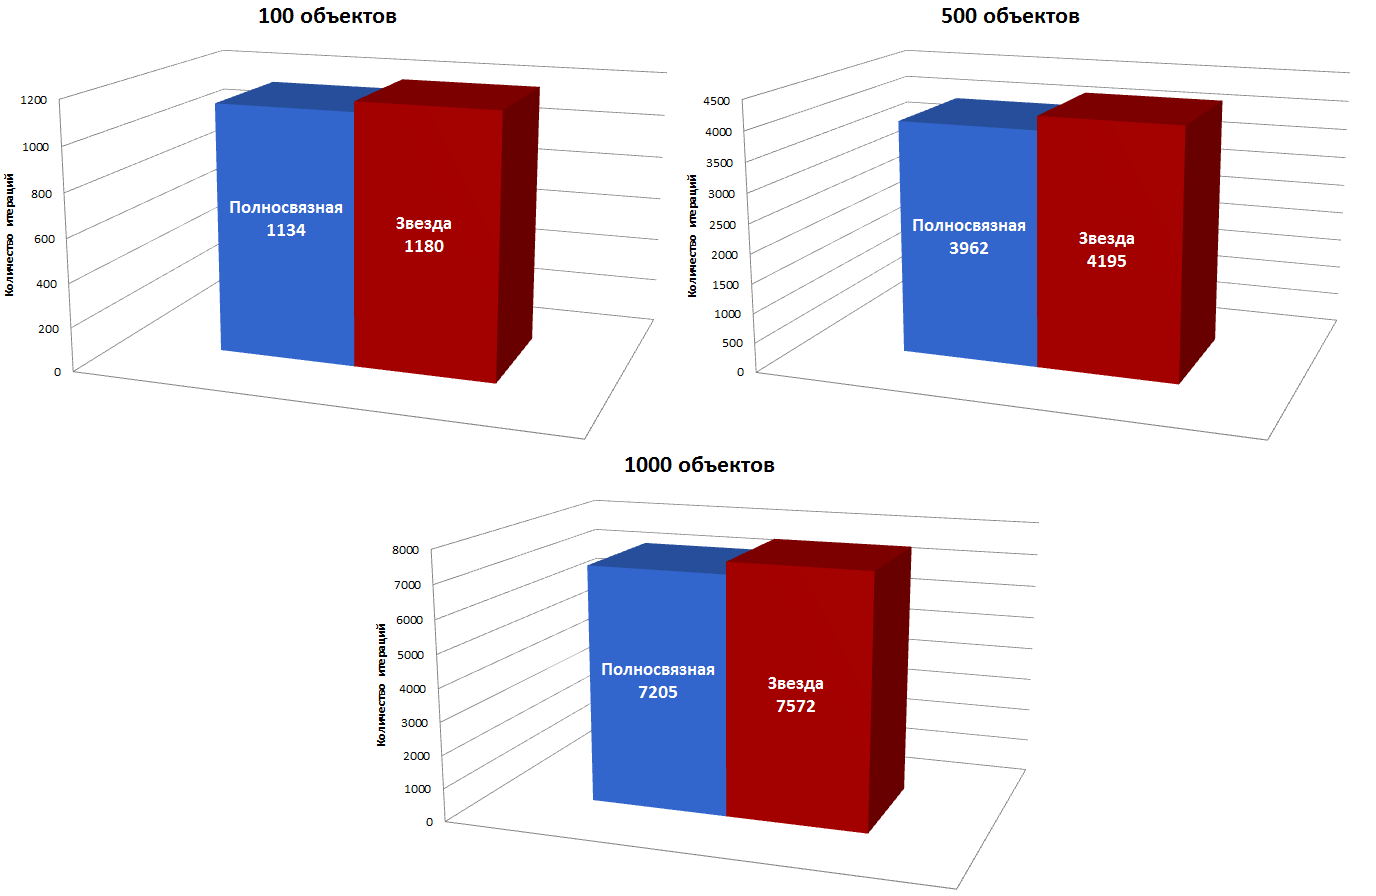
\includegraphics[scale=0.2]{img/histograms/top.png}
		\caption{Влияние топологии сети на количество итераций алгоритма}
	\end{figure}
\end{frame}

\begin{frame}[fragile]{Тестовые испытания}
	\begin{figure}
		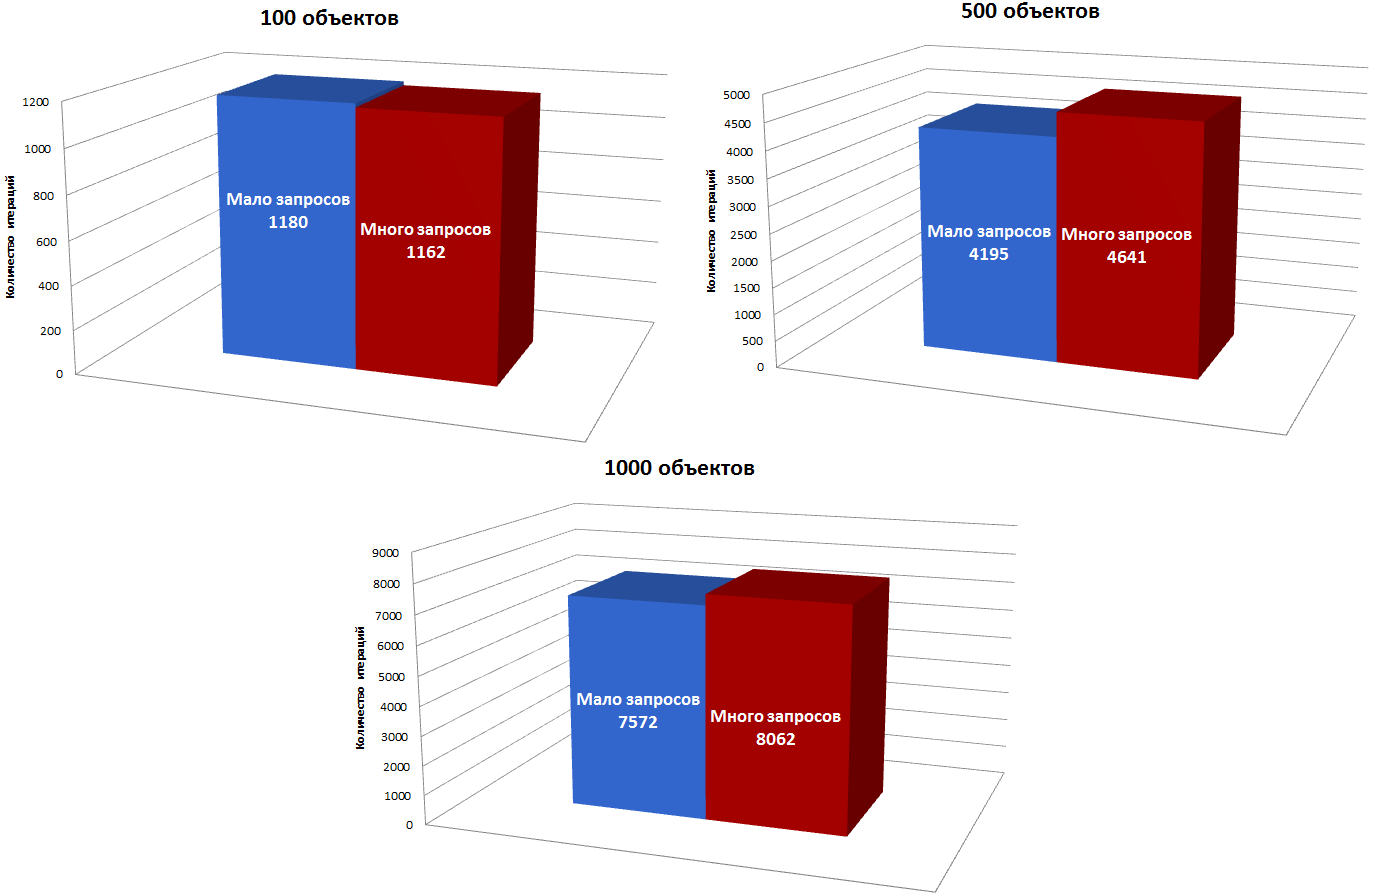
\includegraphics[scale=0.2]{img/histograms/req.png}
		\caption{Влияние общего количества запросов к объекту на количество итераций алгоритма}
	\end{figure}
\end{frame}

\begin{frame}[fragile]{Тестовые испытания}
	\begin{figure}
		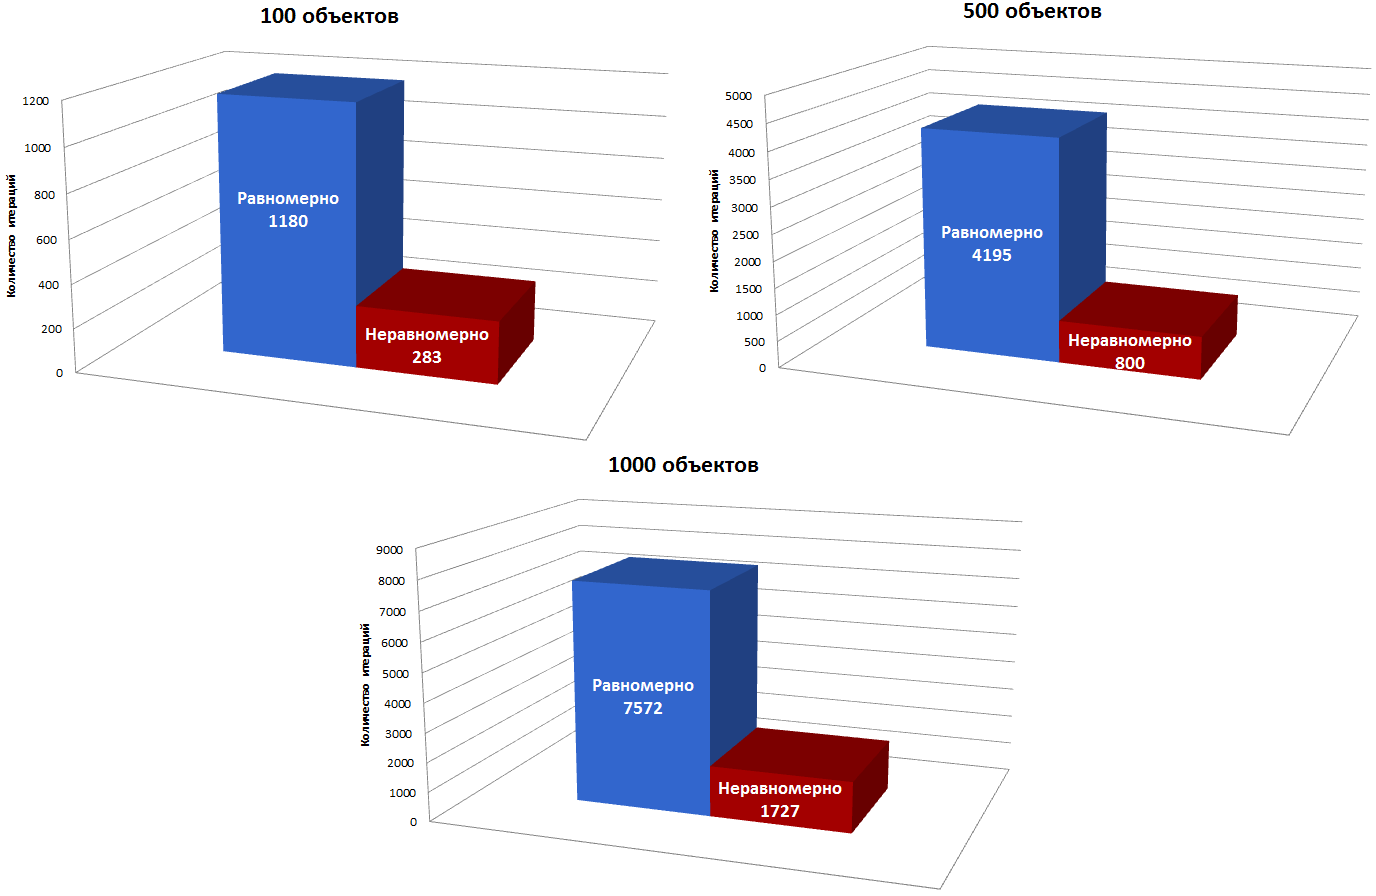
\includegraphics[scale=0.2]{img/histograms/dist.png}
		\caption{Влияние распределения запросов к объектам на количество итераций алгоритма}
	\end{figure}
\end{frame}


% Полученные результаты
\begin{frame}{Полученные результаты}
	\begin{itemize}
		\item Реализовано распределенное клиент-серверное приложение для хранения данных на языке программирования Erlang. 
    	\item Реализован алгоритм размещения реплик объектов в распределенной сети. 
    	\item Проведены замеры количества итераций алгоритма и проанализированы полученные результаты.
	\end{itemize}
\end{frame}

\end{document}
